% !TEX encoding = UTF-8 Unicode

\documentclass[10pt,reqno]{amsart}
\usepackage[russian]{babel}
\usepackage[utf8]{inputenc}
\usepackage{geometry}
\geometry{verbose,a4paper,tmargin=2cm,bmargin=2cm,lmargin=2.5cm,rmargin=1.5cm}
%\usepackage[dvips]{graphicx,graphics}
\usepackage{graphicx}
\usepackage{euscript}
\usepackage{graphics}
\usepackage{centernot}
%\usepackage{russcorr}
\usepackage[active]{srcltx} % SRC Specials: DVI [Inverse] Search
\usepackage{amssymb,amsmath,amsthm,amsfonts}
\usepackage{amsopn}
\newtheorem{cor}{Следствие}
\newtheorem{lem}{Лемма}
\newtheorem{thm}{Теорема}
\newtheorem{prop}{Предложение}
\newtheorem*{thm_pres}{Теорема}
\theoremstyle{definition}
\newtheorem{defn}{Определение}
\newtheorem{defneq}{Эквивалентное определение}
\theoremstyle{remark}
\newtheorem*{rem}{Замечание}
\newtheorem*{deff}{Обозначение}
\newtheorem{ex}{Пример}
\usepackage{verbatim}
\usepackage{listings}
\usepackage{verbatim}
\usepackage{tabularx}
\usepackage{pbox}
\usepackage{bussproofs}

\newcommand{\lfrac} [2] {\displaystyle \frac{#1}{#2}}
\newcommand{\brsum} [3] {\displaystyle \sum \limits_{#1}^{#2} \left( #3\right)}
\newcommand{\lsum} [2] {\displaystyle \sum \limits_{#1}^{#2}}
\newcommand{\br} [1] {\left( #1 \right)}
\usepackage{a4wide}
\begin{document}
\section{Word2Vec}

Word2Vec -- модель, которая по заданному набору текстов, обучает векторные представления для слов с помощью нейронной сети. Все вектора соответствующие словам получены так, что бы максимизировать логарифм вероятности нахождения слова рядом со своими соседями в предложениях их тестовой выборки.

$$
\lfrac{1}{T} \sum_{t = 1}^{T} \sum_{j \in nb(t)} \log{p(w_j | w_t)}
$$

где $nb(t)$ -- это множество всех "соседей" для слова $w_t$.


Если обучить данную модель на достаточно больших датасетах то полученные вектора будут обладать способностью обнаруживать достаточно сложные зависимость, наприпер vec(Japan) - vec(sushi) + vec(Germany) $\approx$ vec(bratwurst) или vec(Einstein) - vec(scientist) + vec(Picasso) $\approx$ vec(painter)

Обучается данная модель без учителя -- что является большим плюсом.

\section{Word Mover’s Distance}

Пусть нам дан некоторый набор текстов в котором n уникальны слов(предполагаем что изначально мы удалили стоп слова). Представим его в виде нормированного мешка слов(nBOW) -- то есть в виде вектора $d \in \mathbb{R}^{n}$, где если i-ое слово встречалось в тексте один раз то  $d_i = \lfrac{c_i}{\sum^{n}_{j = 1}c_i}$.

Представим наш вектор $d$ как точку в $(n - 1)$ мерном симплексе -- рассмотрим следующий пример семантически близких предложений с абсолютно разными словами:

$$
\text{Obama speaks to the media in Illinois}
$$

$$
\text{The President greets the press in Chicago}
$$

$$
w = ['Obama', 'speaks', 'media', 'Illinois', 'President', 'greets', 'press', 'Chicago']
$$

$$
d = [1,1,1,1,0,0,0,0]
$$

$$
d' = [0,0,0,0,1,1,1,1]
$$

После удаления из этих предложений стоп слов вектора $d$ и $d'$ получаются совершенно различны -- они не имеют совершенно никаких общих не нулевых элементов(с учетом из позиции) и даже находятся на почти максимальном расстоянии в симплексе.


Получается что наша задача заключается в том что бы учесть в нашей метрике близости текстов так же и семантическую близость отдельных пар слов. Мера семантической("смысловой") близости слов может быть получена с помощью рассмотрения евклидова расстояния между словами в пространстве в котором находятся вектора полученные путем обучения модели word2vec.


Пусть у нас есть матрица векторных представлений слов из word2vec $X \ in \mathbb{R}^{dxn}$ для n слов конечного размера. B данной матрице каждый столбец $x_i \in \mathbb{R}^{d}$ является векторным представлением i-ого слова.

Тогда расстояние между словами i и j может быть измерено как $c(i, j) = \|x_i - x_j \|_2$  -- стоимость перехода одного слова в другое.


Таким образом мы сделали первый шаг для вычисления расстояния между документами.


Пусть $d$ и $d'$ nBOW представления двух текстовых документов в $(n - 1)$ мерном симплексе. В первую очередь мы должны как то "перевести"  каждое слово из $d$ в какие то слова из $d'$.

Рассмотрим матрицу разряженную матрицу перемещений  $T \in \mathbb{R}^{nxn}$, где $T_{ij} \geq 0$ обозначает как далеко надо переводить слово $i$ из $d$ в слово $j$ из $d'$. Для полного переведения $d$ в $d'$ мы должно выполняться следующее -- количество переводов слова i из d должно быть равно $d_i$ то есть $\sum_{j} T_{ij} = d_i$ и в обратную сторону -- количество переводов слова j из $d'$ должно быть равно $d'_j$ то есть $\sum_{i} T_{ij} = d'_j$. То есть $T_{ij}$ это "количество" слова $i$ из $d$ переходит в слово $j$ из $d'$.

Таким образом мы можем определить расстояние между текстами как минимальную совокупную стоимость перехода требуемую для того чтобы перевести $d$ в $d'$ -- $\min \sum_{i,j} T_{ij} c(i,j)$.


\section{Оптимизационная задача}

Формально данная задача минимизации стоимости перехода из $d$ в $d'$ записывается следующим образом:

$$
\min_{T \geq 0} \sum_{i,j} T_{ij} c(i,j)
$$

$$
\sum_{j = 1}^n T_{ij} = d_i \forall i \in {1, ..., n}
$$

$$
\sum_{i = 1}^n T_{ij} = d_j \forall j \in {1, ..., n}
$$

Данная задача это частный случай задачи earth mover’s distance metric -- известной так же как Метрика Васерштейна, хорошо изученной -- т.е для данной задачи есть методы решения.



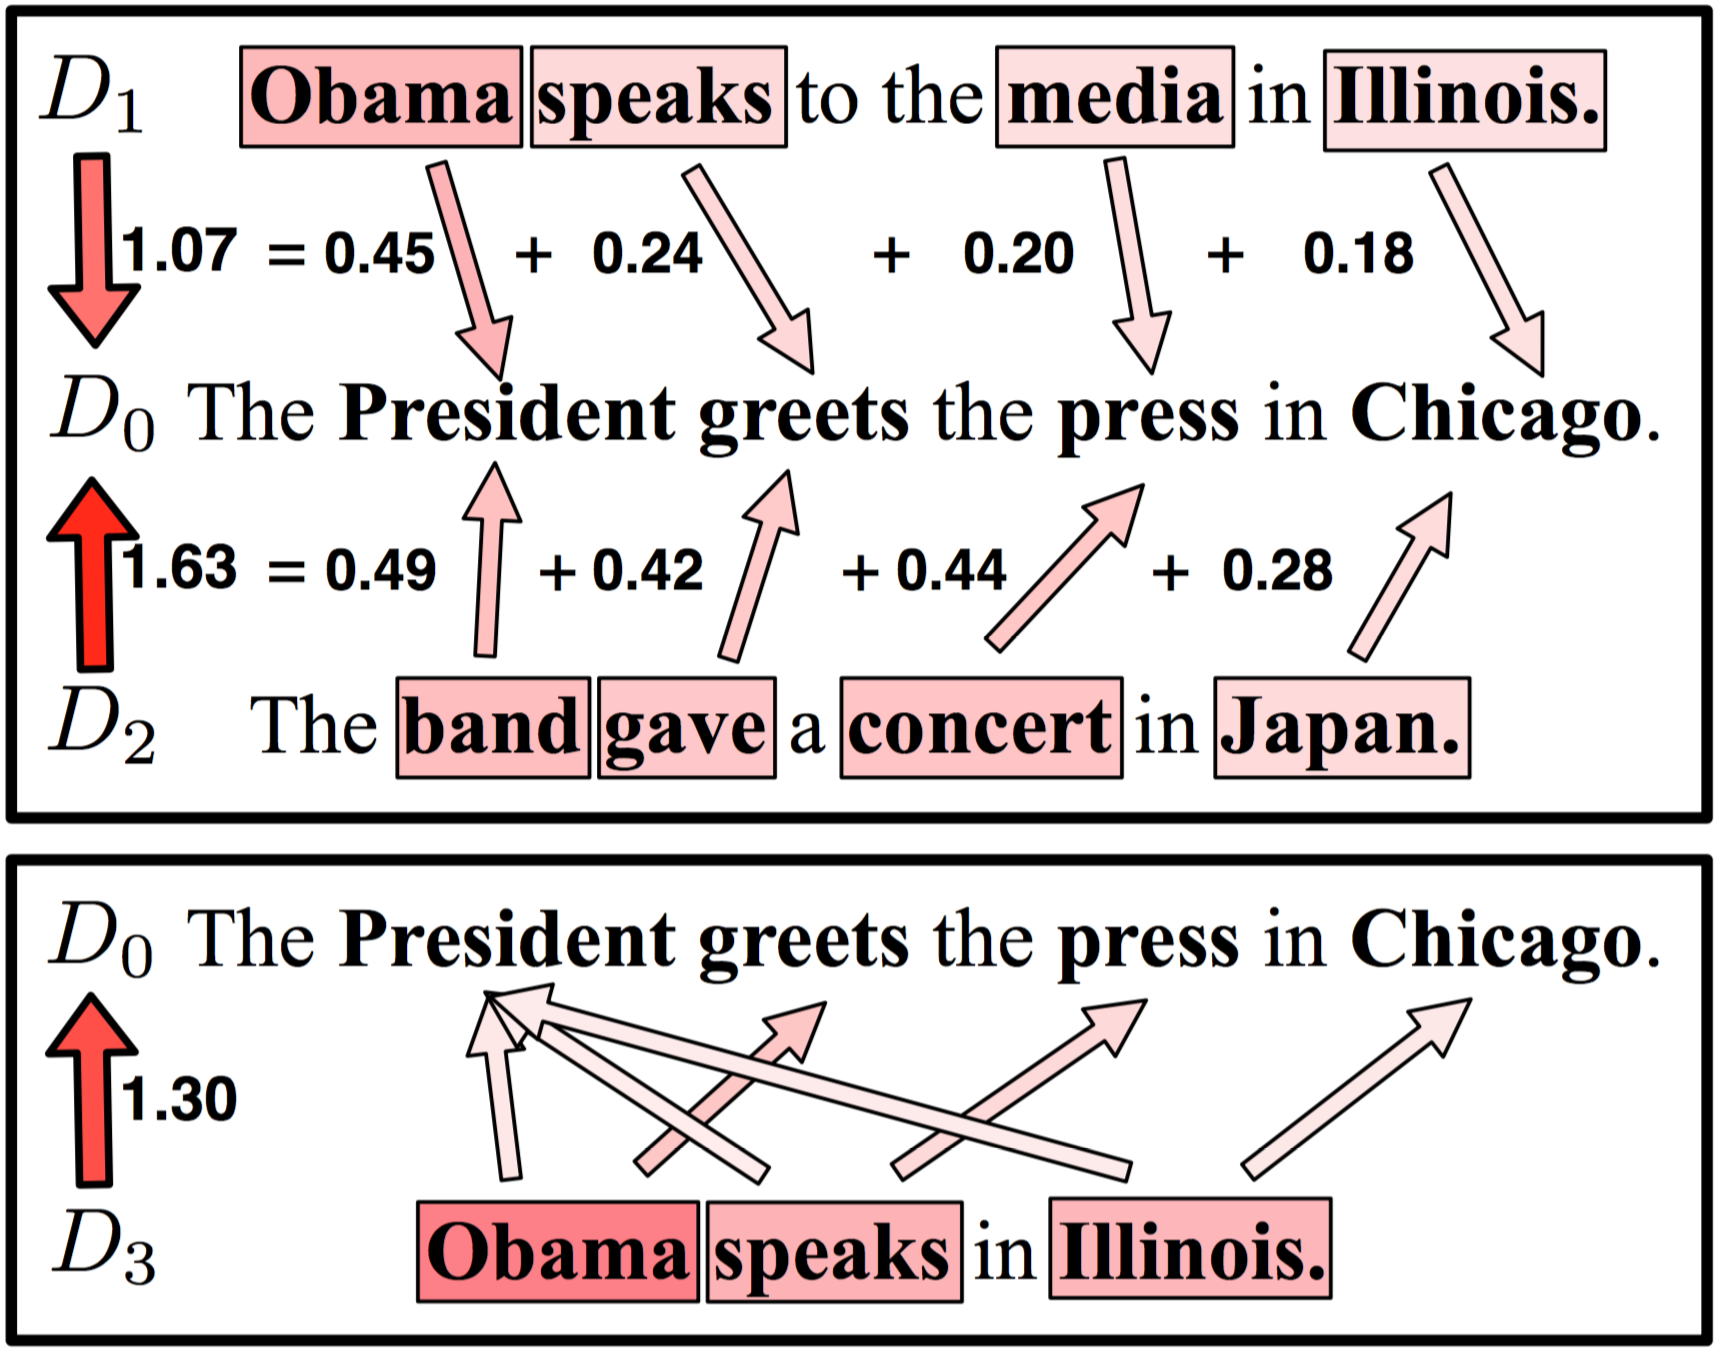
\includegraphics[width=0.8 \textwidth]{1.png}

Рассмотрим работу данной метрики на примере с картинки. В данном примере мы сравниваем предложение $D_0$ с $D_1$ и $D_2$. Для начала из них были удалены стоп слова. Стрелки из каждого слова предложений $D_1$ и $D_2$ подписаны вкладом в расстояние $T_{ij}c(i,j)$. Видно что метрика соответствует нашим ожиданиям и перенесла слова с семантически близкие к ним. Перевод слова Illinois в Chicago гораздо дешевле чем  Japan в Chicago потому что вектора Illinois в Chicago находятся ближе чем Japan в Chicago. Видно что переход из $D_1$ в $D_0$  гораздо дешевле чем в $D_2$ в то время как расстояние рассчитанное через BOW или TF-IDF для $D_0$ с $D_1$ одинаково.

Второй пример показывает как работаешь меток когда число слов в предложениях разные, это увеличило расстояние между словами но такое эффект вызван тем что у нас маленькие предложения и не содержат одинаковых слов.

\section{Оценка сложности задачи}

Оценка сложности получения лучшего решения задачи равна $O(p^3log p)$ где p -- количество различных слов в тексте(взята из решения отптимизационной задачи earth mover distance). В больших датасетах количество уникальных слов велико -- что делает вычисление метрики долгим и проблематичным. Поэтому давайте попробуем как то оценивать эту метрику с помощью нижней границы.


\section{Word centroid distance}

Рассмотрим следующую нижнуюю границу:

$$
\sum_{i,j=1}^n T_{ij} c(i,j) = \sum_{i,j=1}^n T_{ij} \|x_i - x'_j \|_2 = \sum_{i,j=1}^n \|T_{ij} (x_i - x'_j) \|_2 \geq
$$

$$
\geq \| \sum_{i,j=1}^n T_{ij} (x_i - x'_j) \|_2 = \| \sum_{i=1}^n \left(\sum_{j=1}^n T_{ij}\right) x_i - \sum_{j=1}^n \left(\sum_{i=1}^n T_{ij}\right) x'_j \|_2 =
$$

$$
= \| \sum_{i=1}^n d_i  x_i - \sum_{j=1}^n d_j x'_j \|_2 = \| Xd - Xd'\|_2
$$

Даная метрика называется Word Centroid Distance (WCD) в ней для каждый документ представлен средними весами вектора слов. Сложность данного метода $O(dp)$ -- что очень мало. Используя данную метрики можно классифицировать тесты алгоритмом knn на больших датасетах потому что она достаточна быстрая в плане вычисления или же ее можно использовать для того что бы отсеять совсем дальних соседей а дальше уже воспользоваться точной метрикой.

\section{Relaxed word moving distance.}

Несмотря на то что WCD очень быстра для вычисления, она не очень хорошо оценивает нашу метрику. Мы можем получить гораздо более лучшую оценку при ослаблении условий оптимизации с помощью удаления одного из условий(removing both constraints results in the trivial lower bound T = 0).

$$
\min_{T \geq 0} \sum_{i,j} T_{ij} c(i,j)
$$

$$
\sum_{j = 1}^n T_{ij} = d_i \forall i \in {1, ..., n}
$$

Данная задача оптимизации помогает получить нижнюю оценку WMD. Видно что любое  решение основной оптимизационной задачи также будет решением упрощенной. Тогда оптимальное решение для каждого слова из $d$ это перемещение в самые похожие слова из $d'$. Таким образом оптимальное решение данной задачи следующее:

$$
T^*_{ij} =
\begin{cases}
	d_i if j = \text{argmin}_j c(i,j)
	0 otherwise
\end{cases}
$$

Оптимальность данной матрицы легко показать. Пусть $T$ любой матрицей являющейся решением лдя данной задачи, тогда вклад в занчение для любого слова не может быть меньше $j* = \text{argmin}_j c(i,j)$:

$$
\sum_{j} T_{ij} c(i,j) \geq \sum_{j} T_{ij} c(i,j*)  =   c(i,j*) \sum_{j} T_{ij} = c(i,j*) d_i = \sum_{j} T^*_{ij} c(i,j)
$$

Вычислительно данная метрика требует только вычисление $j* = \text{argmin}_i c(i,j)$ что является поиском наиближайшего соседа в евклидовом пространстве word2vecа. Для каждого вектора $x_i$ из документа $D$  нам нужно найти самый ближнвй к нему вектор $x_j$ из $D'$.

Второй вариант - когда снимается второй ограничение практически идентичен, просто задача поиска ближайшего соседа оборачивается в обратную сторону. Обе границы можно посчитать одновременно и это будет иметь не такую уж и большую сложность. Обозначим это границы $l_1(d, d')$ и $l_2(d, d')$ соответственно. Мы можем получить лучшею оценку взяв максимум от этих двух границ -- $l_r(d, d') = max(l_1(d, ,d'), l_2(d, d'))$ -- такая оценка называется Relaxed WMD (RWMD). Данная оценка значительно лучше чем WCD. Оценка сложности алгоритма knn на данной метрике равна $O(p^2)$

Мы можем использовать полученные оценки метрики что бы резко сократить количество(сложность) вычислений при нахождении ближайших k соседей для данного документа.

\section{Результаты данной метрики}

Данную метрику проверяли на kNN классификаторе на 8 различных датасетах.

Для начала рассмотрим датасеты на которых проводились эксперименты.

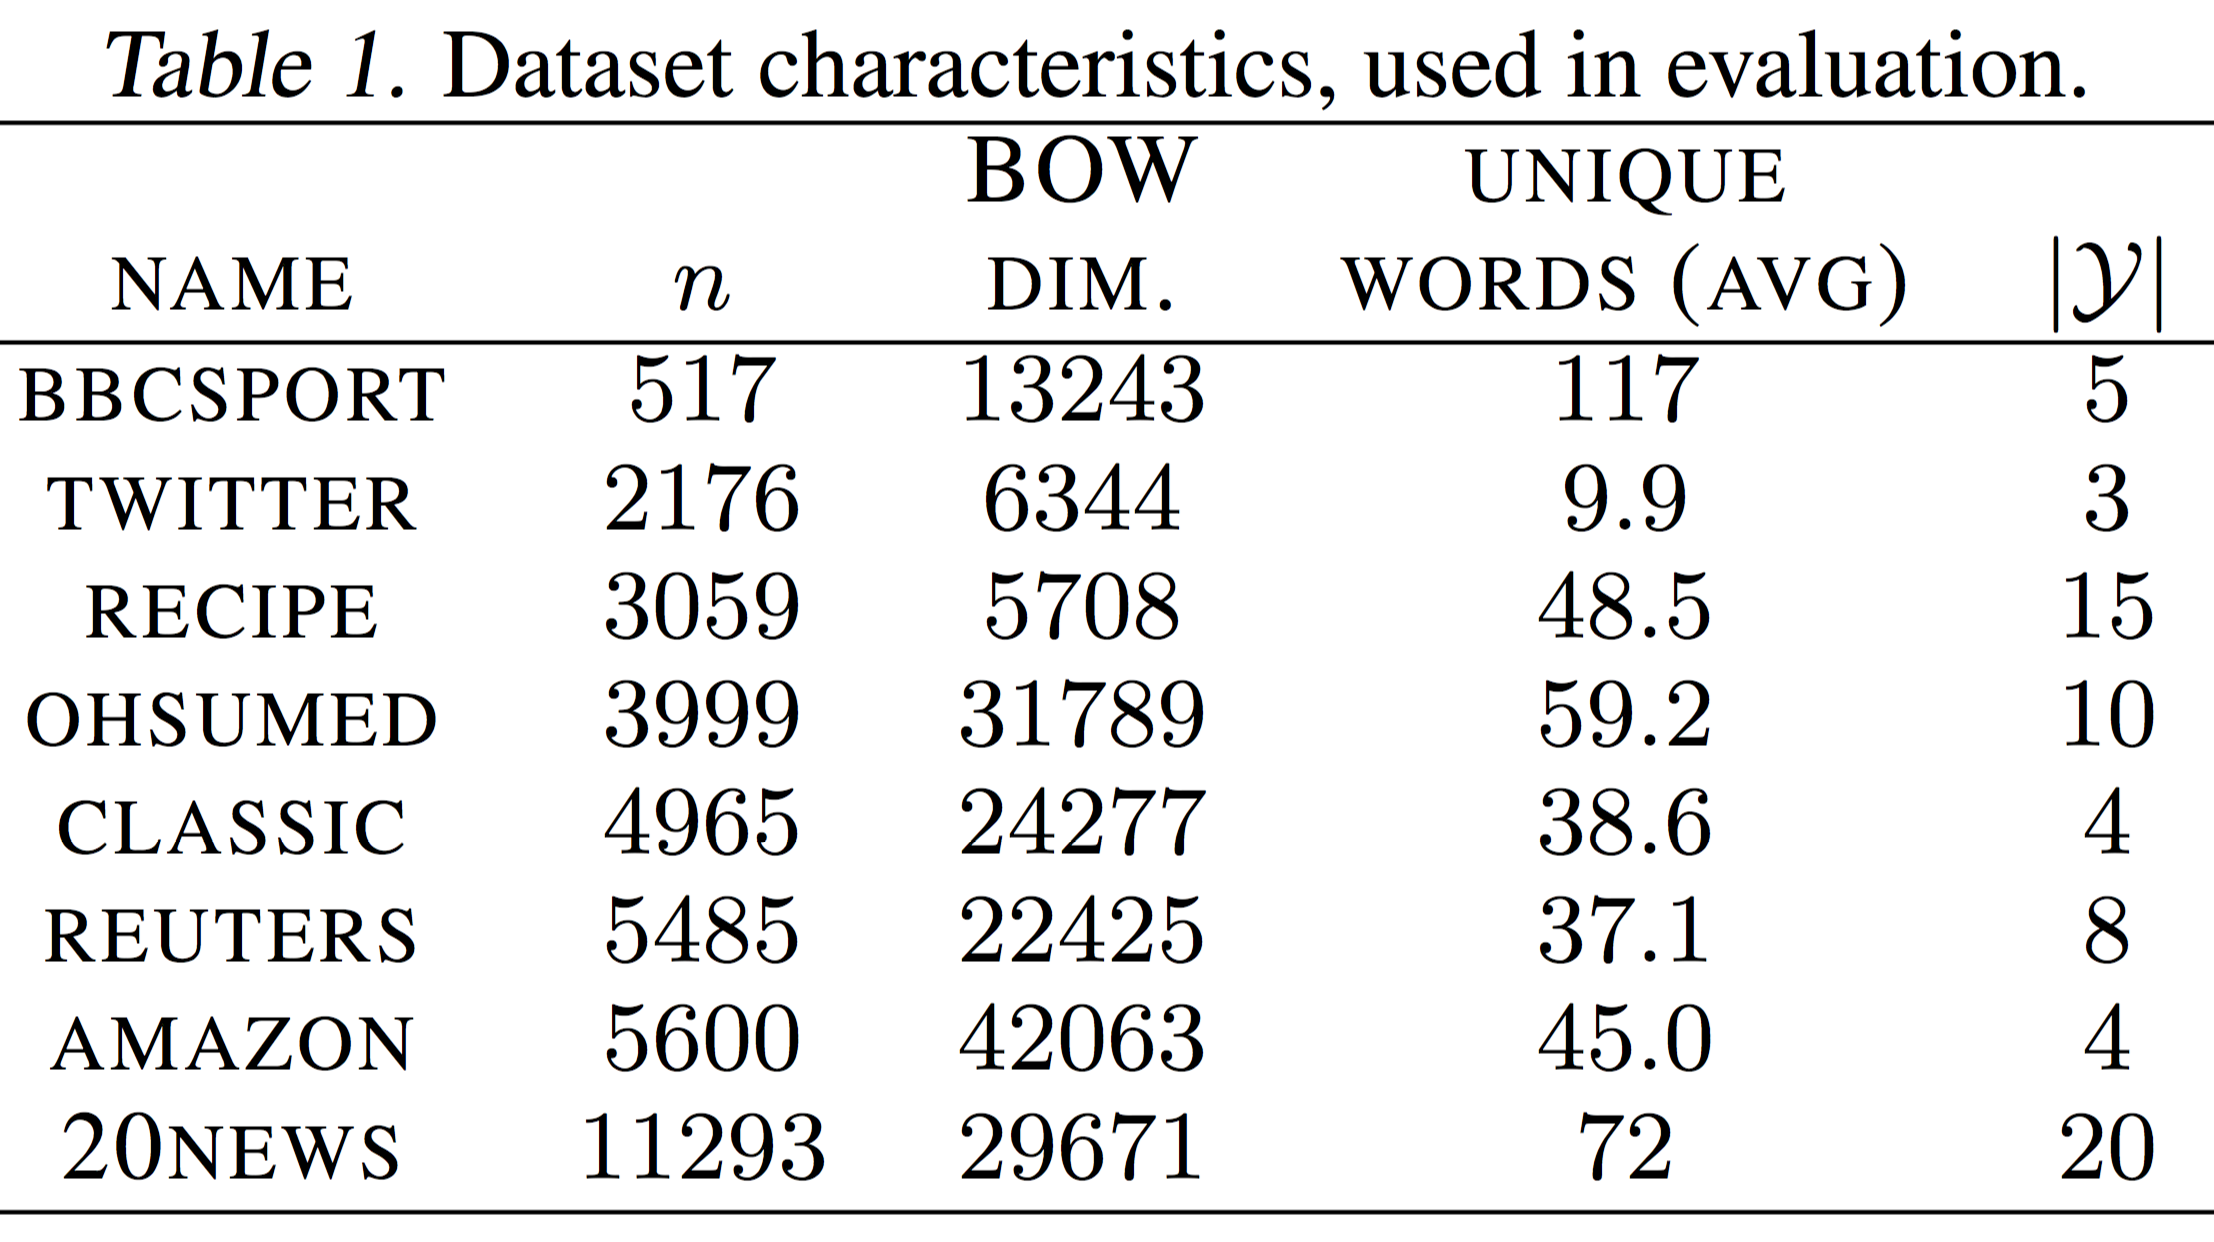
\includegraphics[width=0.6 \textwidth]{2.png}

BBCSPORT -- статьи опубликованные в период с 2004 до 2005 года


TWITTER -- датасет из твитов размеченных как 'позитивные' 'негативные' 'нейтральные'


RECIPE -- набор рецептов размеченных регионом происхождения


OHSUMED -- коллекция медицинских рефератов, отличающиеся различными сердечно-сосудистыми группам заболеваний


CLASSIC -- датасет из наборов предложений из академических статей размеченных именем автора


AMAZON -- датасет отзывов с амазона, которые помечены по категориям продуктов в (книги, DVD, электроника, кухонная)


20NEWS -- набор статей размеченныз на 20 различных категорий


Из всех датасетов были удалены стоп слова. Данная таблица отображает статистику для каждого датасета, количество уникальных слов -- размерность  bag-of-words, среднее количество уникальных слов в документе, и количество классов $|y|$


Использовался  word2vec обученный на 3 миллионах слов/фраз из статей новостей гугла. слова на которых не обучался word2vec были удалены при вычислении метрики.

Для сравнения были взяты 7 бейзлайнов


$\bullet$ bag-of-words


$\bullet$ TFIDF term frequency-inverse document frequency


$\bullet$ BM25 Okapi -- расширенная версия TFIDF


$\bullet$ LSI Latent Semantic Indexing  -- использует сингулярное разложение надо BOW для построения семантического пространства


$\bullet$ LDA Latent Dirichlet Allocation -- генеративная модель для текстовых документов, обучает представления документов как распределене слов в темах темы.


$\bullet$ mSDA Marginalized Stacked Denoising Autoencoder -- обучается несколько автоэнкодера изолированных друг от друга для быстроты обучения.


$\bullet$ CCG Componential Counting Grid -- генеративная модель которая моделирует документы как представление распределений слов


\section{Классификация документов}

Метрики сходства документов для классификации датасетов с помощью kNN метода. Плюс kNN в том что в отличие от других методов его результаты хорошо интерпретируются и могул быть использованы в ранжировании и рекомендательных системах.

Для сравнения вычисления качества решения было использовано евклидово расстояние. Гиперпараметры алгоритмов были подобранны на 80 процентах выборки и итоговое качество считалось на итоговых 20

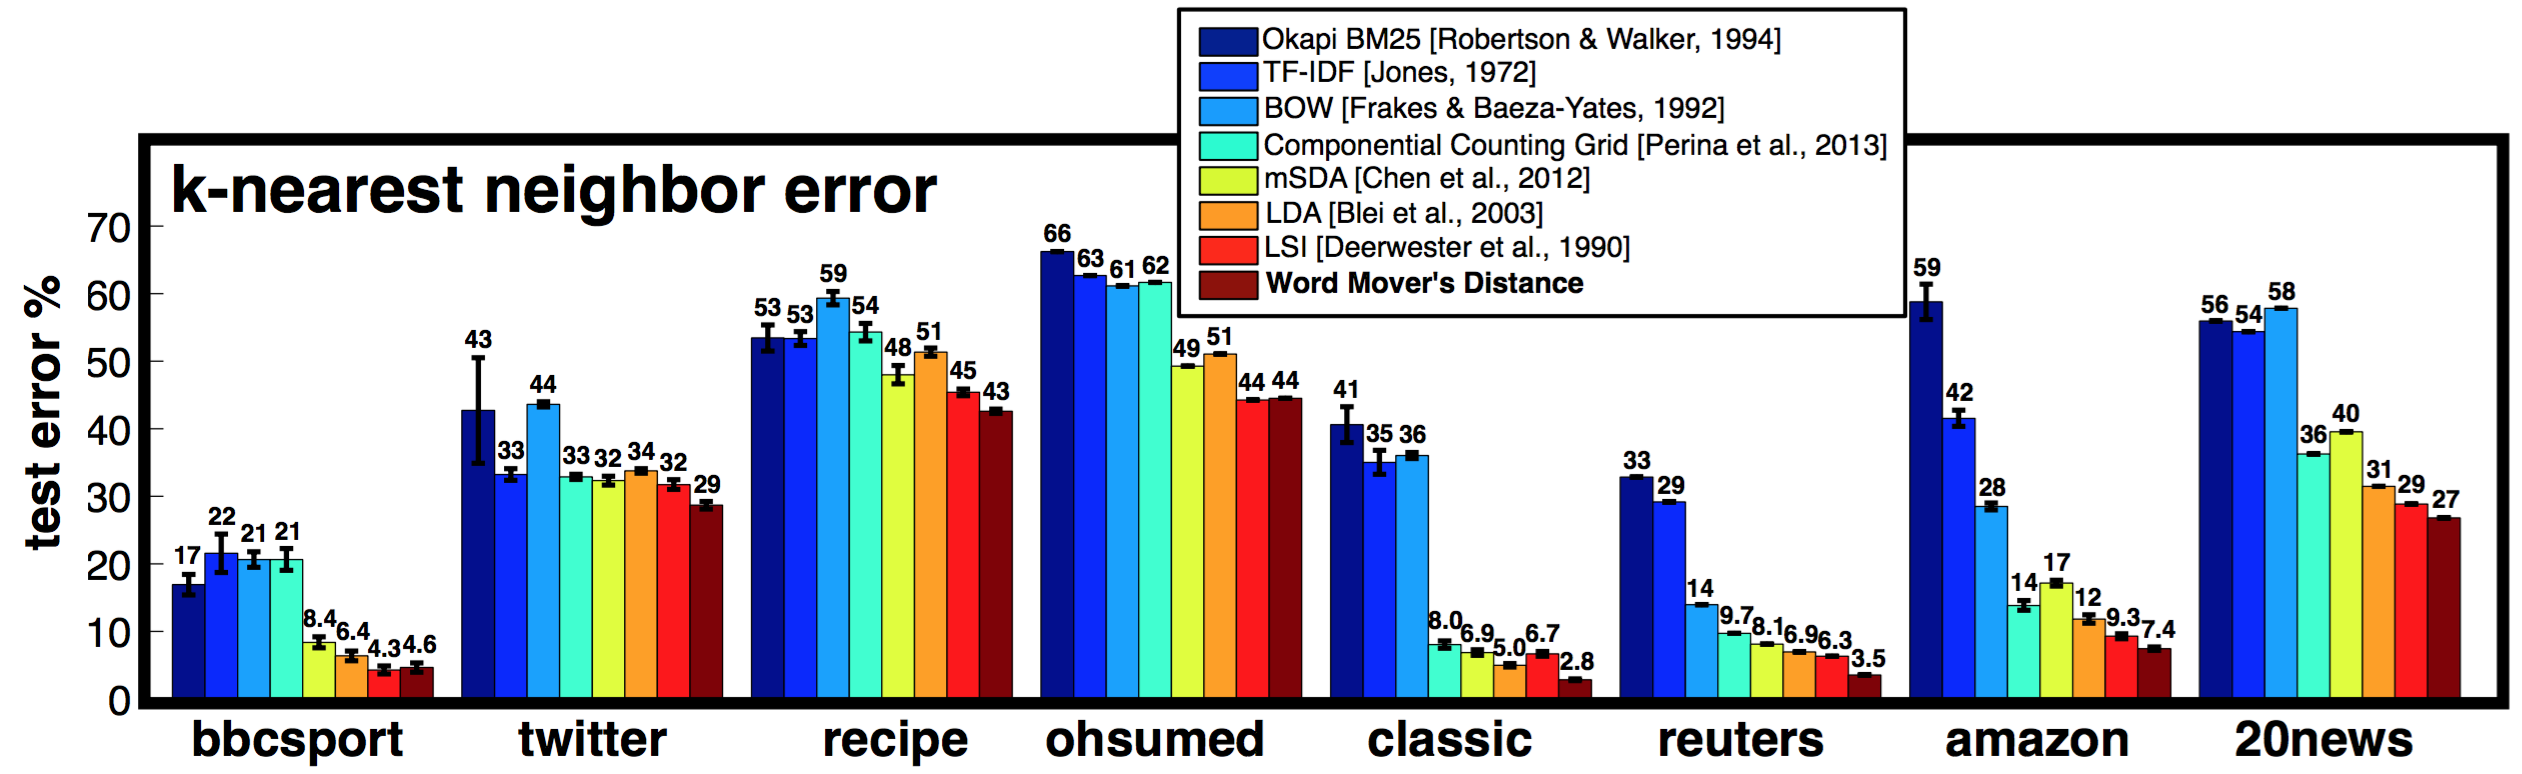
\includegraphics[width=1 \textwidth]{3.png}


Данная таблица показывает ошибку 8 классификаторов на 8 тестовых датасетах. Для алгоритмов которые не требовали предварительного обучения или подбора параметров на трейне, датасеты были разделены на 5 частей и общая ошибка считалась как среднее. Практически на всех датасетах, кроме BBCSPORT, OHSUMED WMD  имеет наименьшую ошибку по сравнению с другими алгоритмами. В частности на датасете TWITTER WMD достигает понижение ошибки аж на 10\%

Одно из возможных объяснений плохого показателя на OHSUMED это то что в данных статьях встречается очень много медицинских терминов которые скорее всего не представлены в word2vec.

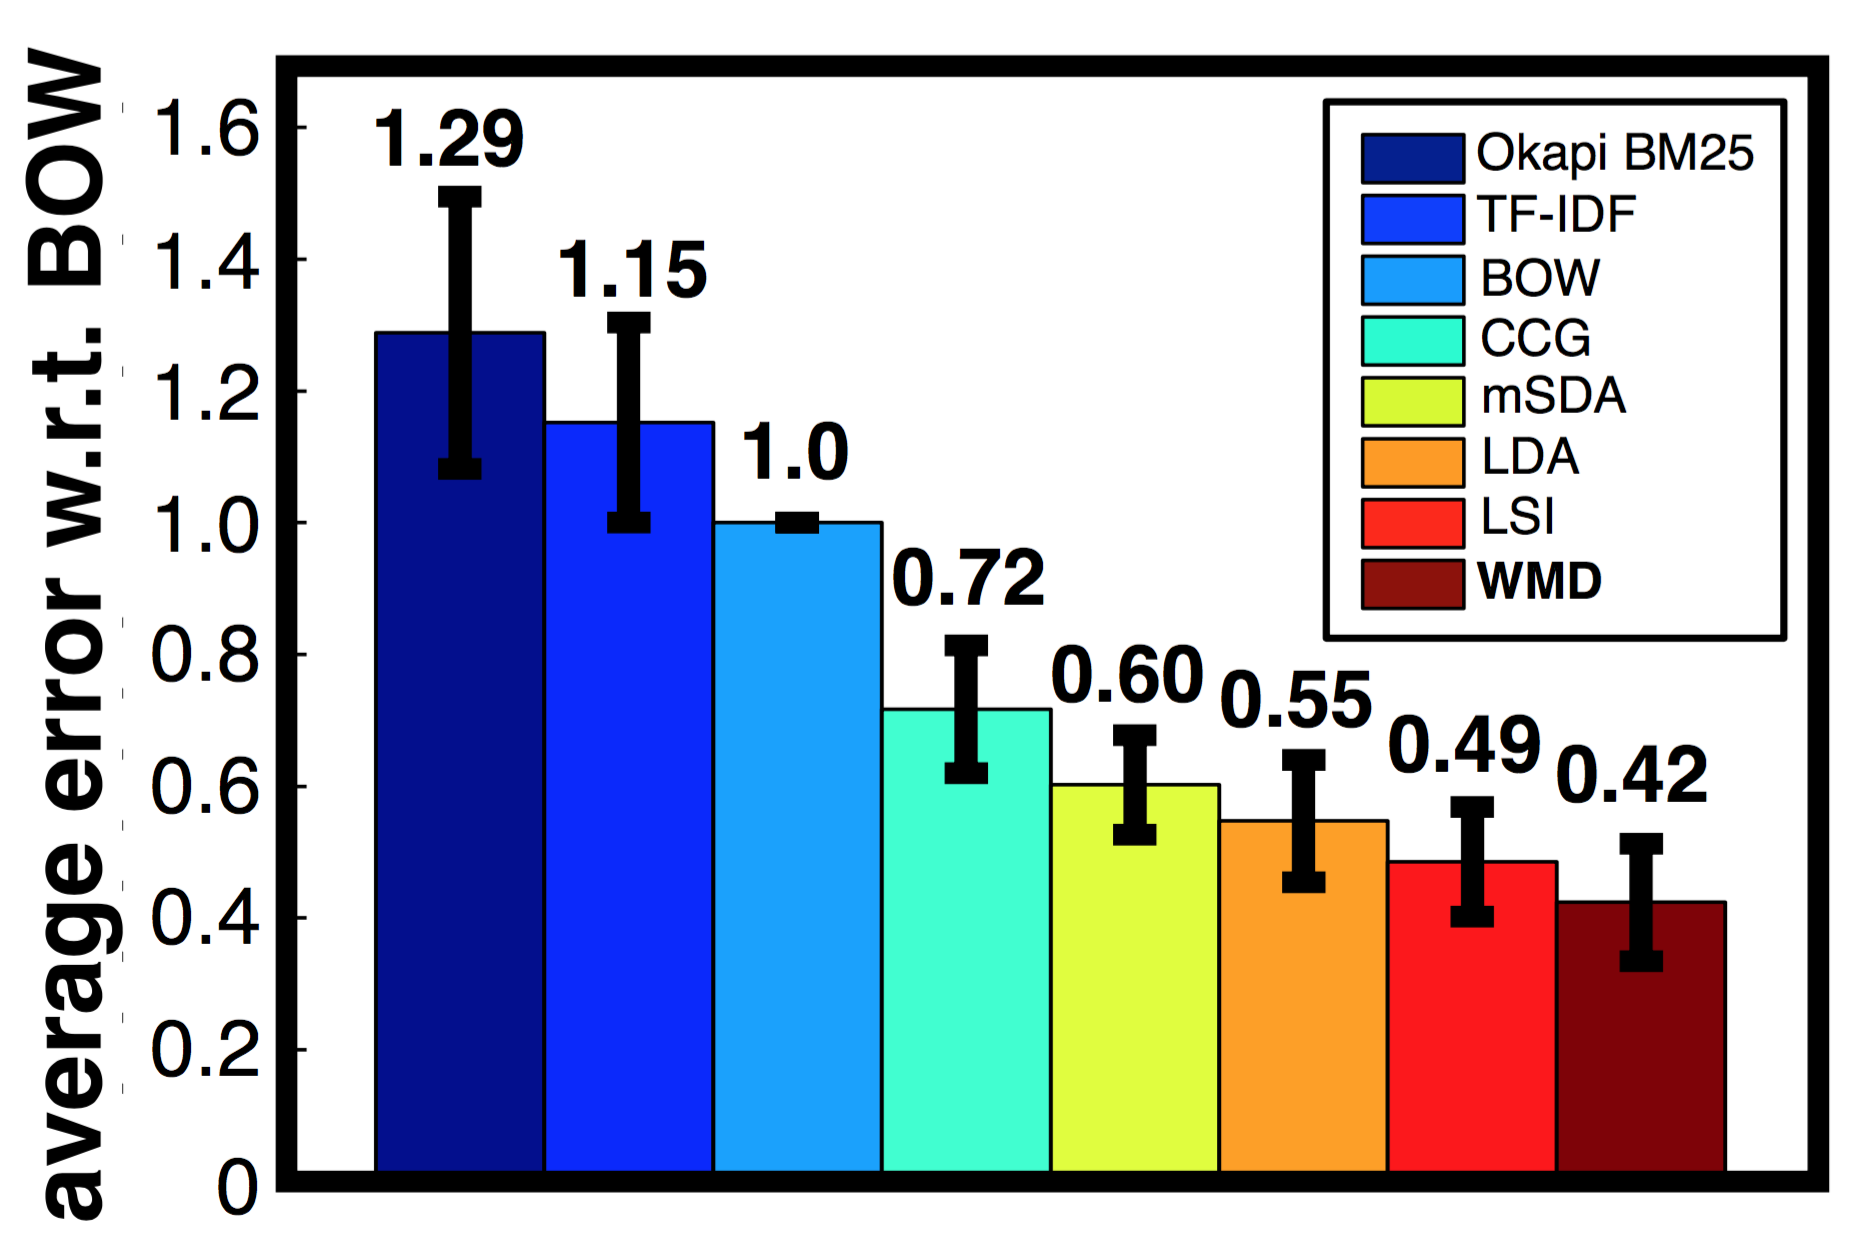
\includegraphics[width=1 \textwidth]{4.png}

На данной картинке показаны среднее увеличение ошибки каждого алгоритма по сравнию с WMD.



\section{Оптимизация kNN}

Заоптимизируем алгоритм kNN под нашу метрику и ее оценки:

$\bullet$ Сортим все документы по возрастанию метрики WCD

$\bullet$ Вычисляем WMD для первых k документа из предыдущего шага

$\bullet$ Проходимся по каждому из m ближайшим документов не вошедших в k и проверяем что если RWMD данного документа меньше расстояния k-ого то мы добавляем его в k ближних, считает для него WMD, сортим все k + 1 и оставляем k.


Посмотрим как ведет себя данный алгоритм на тестовых данных.

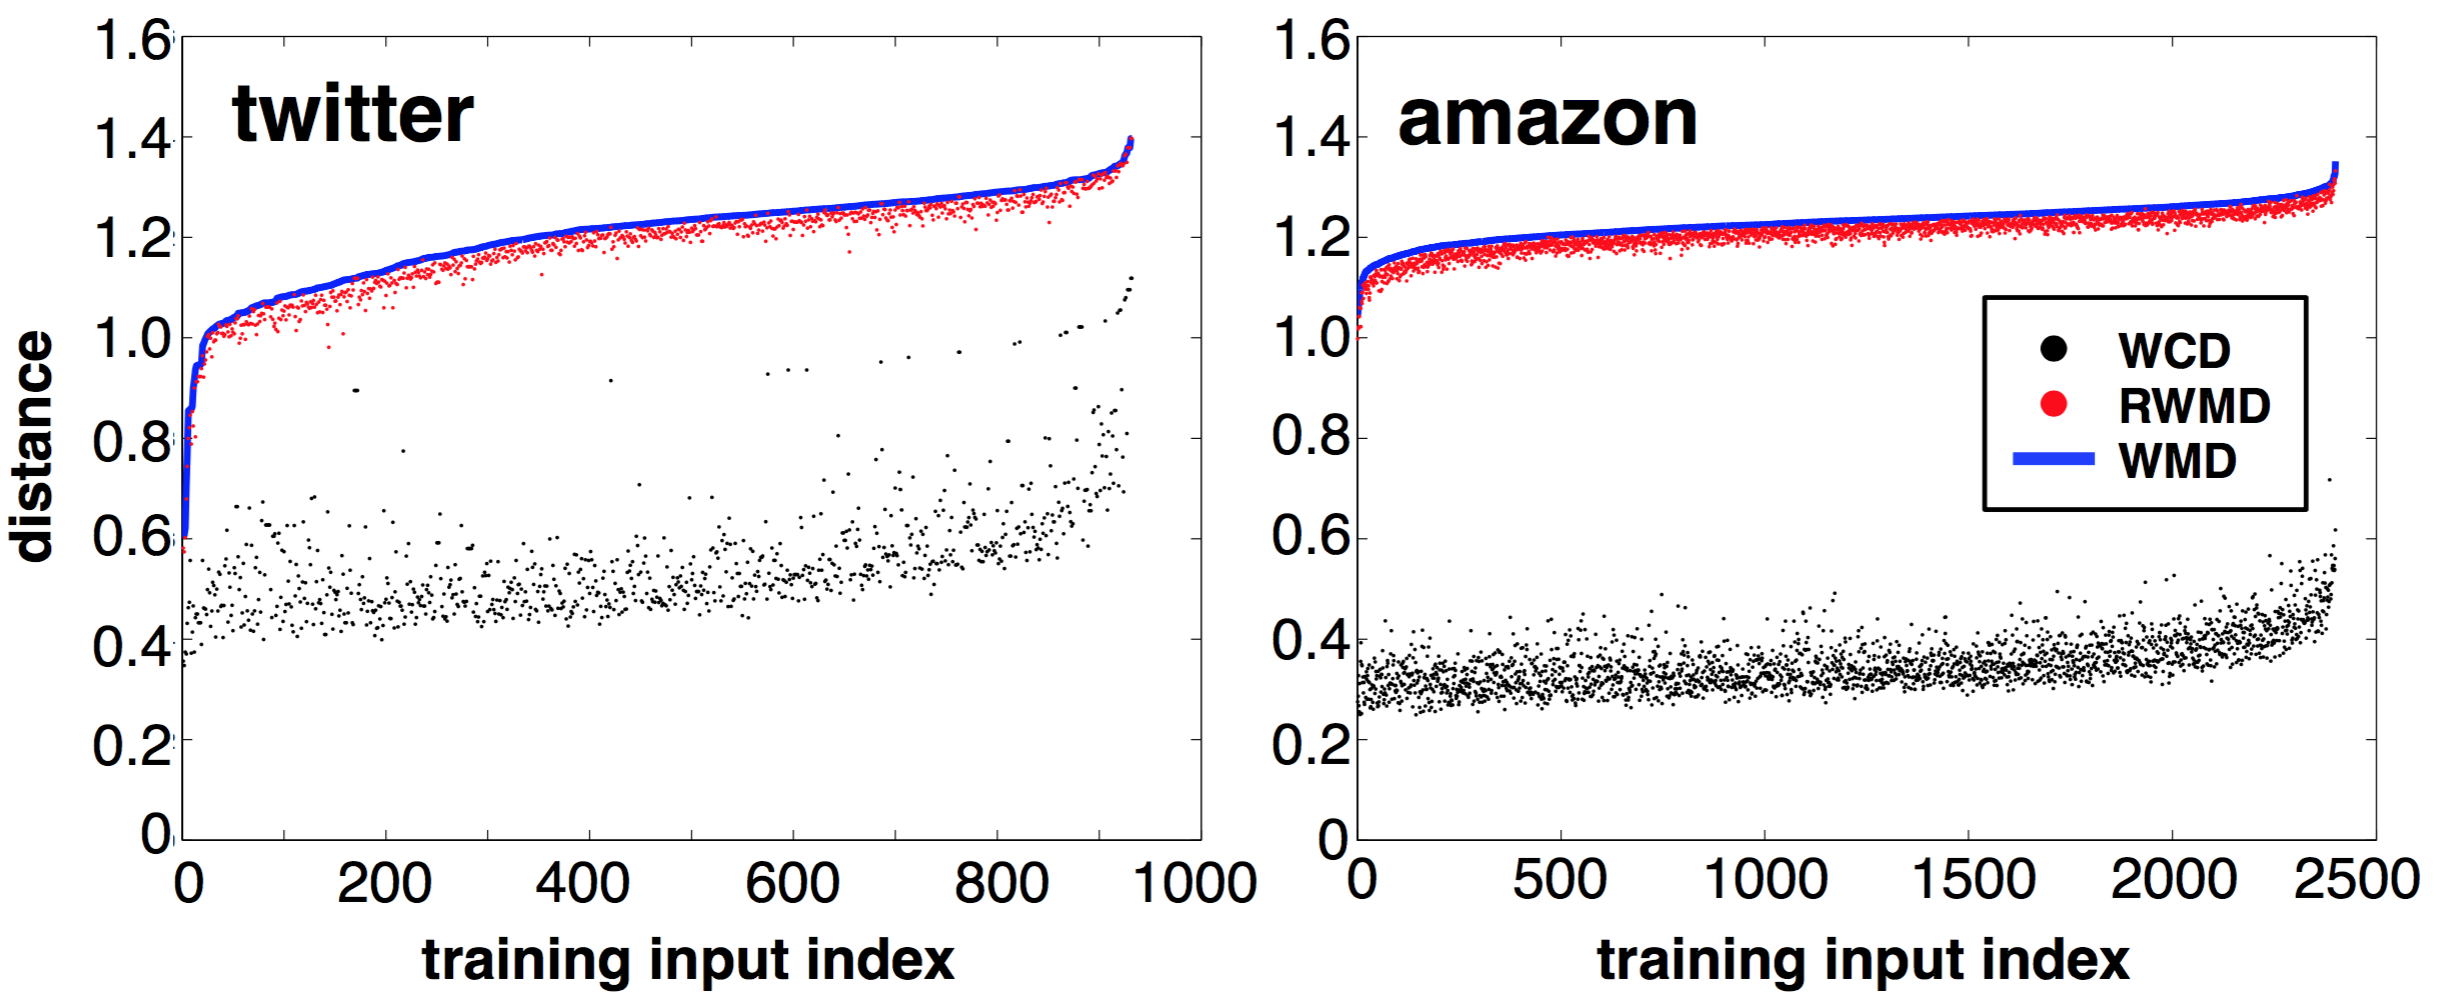
\includegraphics[width=1 \textwidth]{7.png}

На данном графике можно наблюдать насколько точно мы оцениваем нашу метрику. Граница RWMD очень близка к настоящему значению. А граница WCD достаточно рахлая(?) и расположена далеко от реального значения метрики. Но несмотря на это форма этой рыхлой линии в точности повторяет форму линии с реальным значением метрики, что позволяет что делает ее полезной эвристикой для выявления перспективных кандидатов в ближайшие соседи.


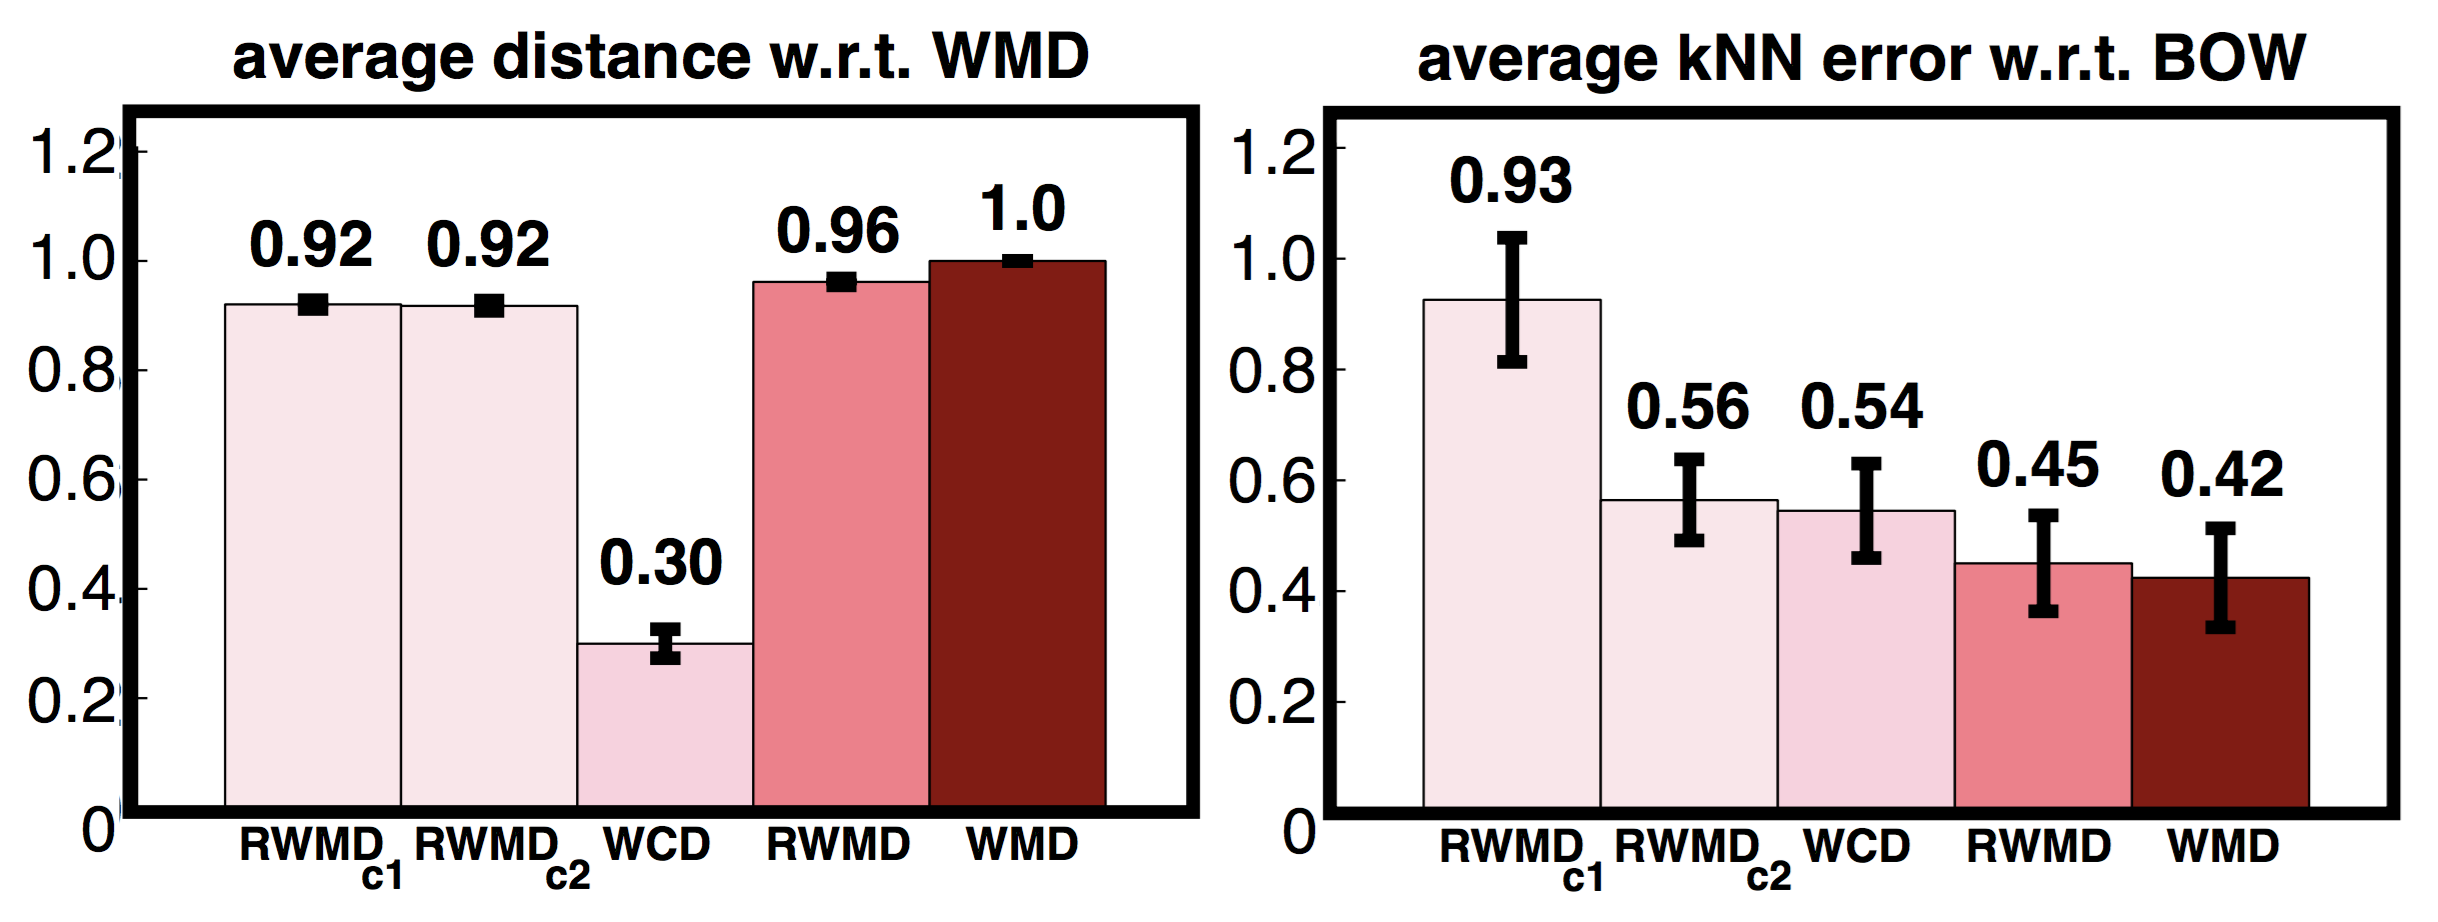
\includegraphics[width=1 \textwidth]{6.png}

Рассмотрим данный график, на первом видно как себя показывают оценки метрики по сравнению с реальной метрикой. Видно что WCD совсем плох. На котором видно что значение ошибки RWMD c1 и c2 работают хуже чем WCD но при этом их композиция лучше. При этом стоит подчеркнуть что средняя ошибка кнн с RWMD попрежнему превосходит все базовые показатели.



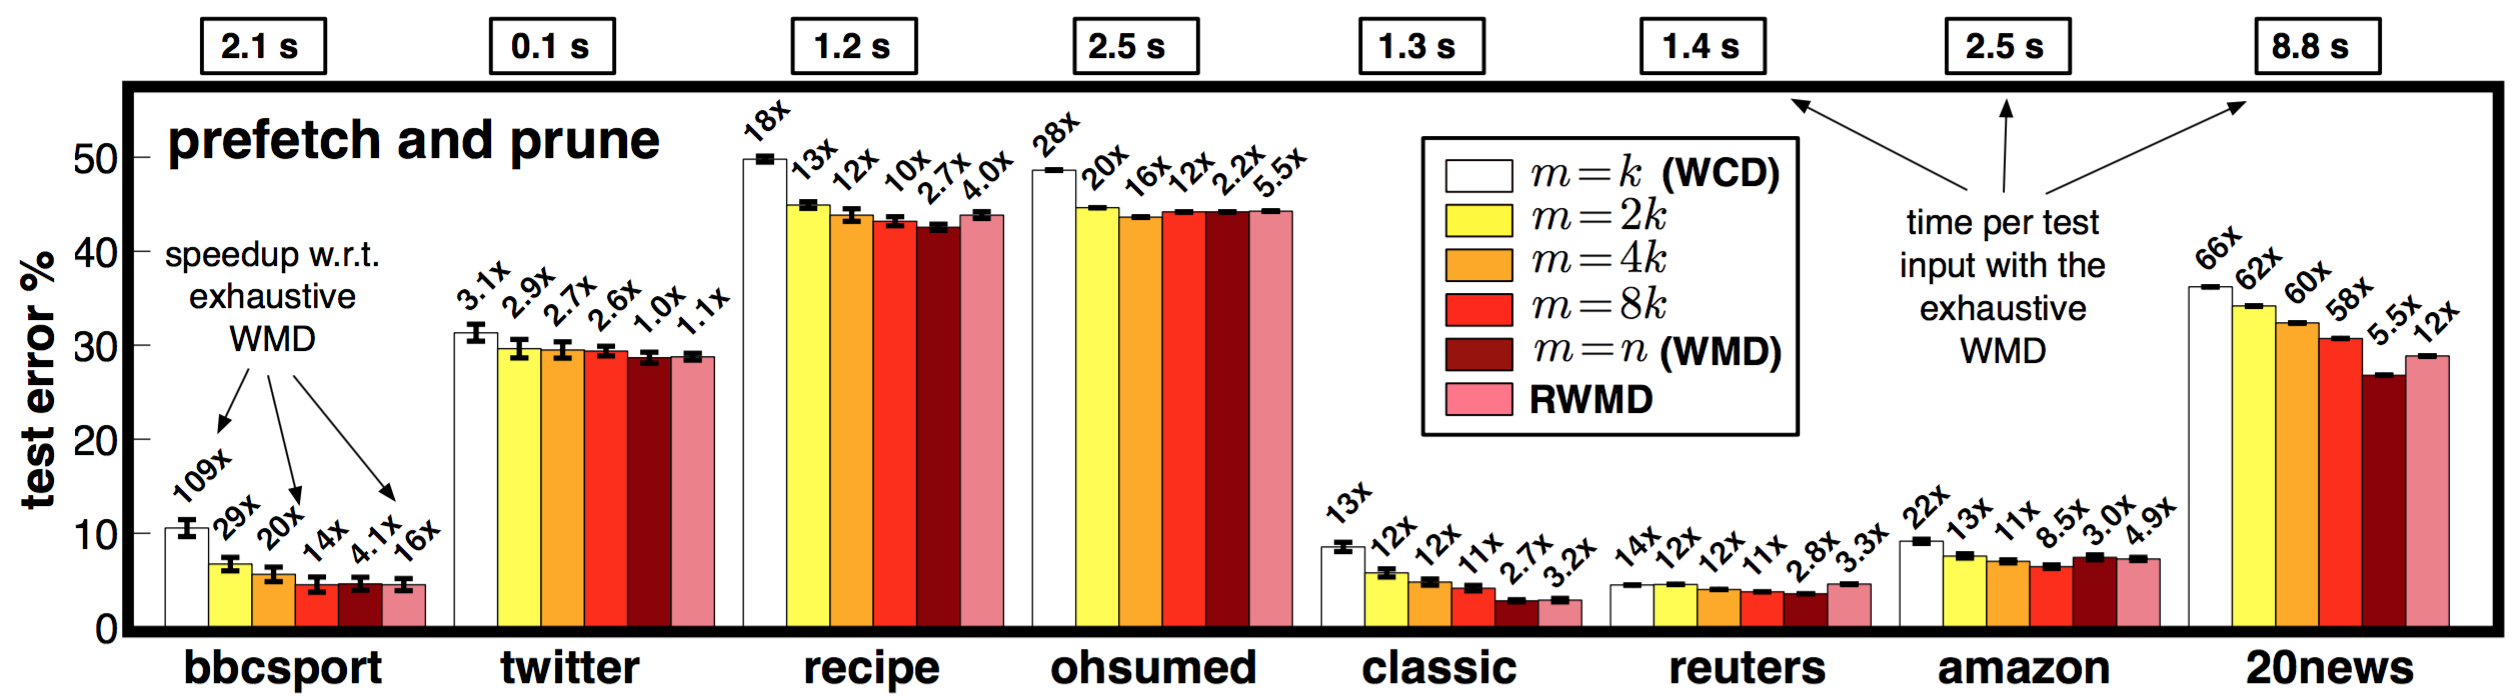
\includegraphics[width=1 \textwidth]{8.png}

Стоит заметить что увеличение ошибки от изменения m  не так существенно. В среднем ошибка минимальна при m=2к
\end{document}
